
\chapter{Doing design (2 of 2)}
\label{design2}

\section{The two domains}

Before we dive back in and complete our two examples from last chapter, let me
make an observation about the classes in an OO program. They tend to come from
two different sources. We call these two categories ``the \textbf{problem
domain}'' and ``the \textbf{solution domain}.''

\index{problem domain}
The problem domain provides classes that relate to the \textit{problem} the
program is designed to solve. A key give-away of a problem domain class is
that the user herself recognizes the term used. She thinks of that entity as
central in what the system does/is.

\index{bid@\texttt{Bid}}
\index{auction@\texttt{Auction}}
\index{item@\texttt{Item}}
\index{seller@\texttt{Seller}}
\index{buyer@\texttt{Buyer}}
\index{eBay}
For instance, in an eBay type application, classes like \texttt{Bid},
\texttt{Auction}, \texttt{Item}, \texttt{Seller}, and \texttt{Buyer} are all
from the problem domain. eBay users think about, and talk about, these very
concepts when they think about the system, even if ``code'' never crosses their
mind.

\index{solution domain}
\index{smtpServer@\texttt{SMTPServer}}
\index{messageListener@\texttt{MessageListener}}
\index{loginPane@\texttt{LoginPane}}
The other source of classes is the solution domain, which consists of
supportive classes that don't really represent things about the problem
itself, but which are necessary to solve the problem. Suppose an email
application had a \texttt{SMTPServer} class. This would represent a connection
to a piece of hardware that acted as a SMTP (Simple Mail Transfer Protocol)
server to deliver electronic mail. Is this class's functionality necessary to
send email, as the email application needs to do? Yes. But does an everyday
email user think about ``SMTP Servers'' being involved? Likely not. The same
could be said of classes like ``\texttt{DatabaseConnection},''
``\texttt{MessageListener},'' and ``\texttt{LoginPane}.''  These classes all
perform critical supporting functions and therefore are vital to the operation
of the system. At the same time, though, we recognize that they are tangential
to the main purpose of the system as the user sees it: users of Wikipedia
don't think in terms of ``database connections,'' nor email users of ``message
listeners,'' nor Spotify users of the ``login panes'' in their UI. So we
relegate those classes to a different realm of sorts; one that contains
classes to perform functions, not to represent the domain's reality.

\index{connection}
\index{Spotify}
\index{song@\texttt{Song}}
\index{playlist@\texttt{Playlist}}
You might wonder which of the two domains is most important to get right. The
answer is unquestionably the \textit{problem domain}. Think about it: if
Spotify decided to change their underlying storage mechanism, and thus
needed to retire their \texttt{DatabaseConnection} class, that's not a big deal to their
user base. If the new program version is implemented well and doesn't
introduce a lot of lagginess or bugs, the user will be unaware that it was
even changed. But change something in the \textit{problem} domain, and whoo
Nellie, the whole system experiences a change. Imagine if Spotify got rid of
their \texttt{Song} or \texttt{Playlist} classes. The entire application would
have to perform differently, with serious consequences for the user.


\section{Turning CRC cards into UML}

\index{CRC card}
When we last left our heroes in chapter~\ref{design1}, they had succeeded in
turning an English language description into a set of CRC cards. That's a ton
of progress. All they need to do now is complete the trick: turn those CRC
cards into a UML class diagram, and then into Java code. And that's just what
we'll do in the rest of this chapter.

\subsection{The bike store example, continued}

\index{CRC card}
Reacquaint yourself with the CRC cards on
pp.~\pageref{bikeCRC1}--\pageref{bikeCRC2}. These reflect some of the candidate
classes from our bike store example.

You've probably already figured out that when turning a CRC card into a class,
the ``Knows:'' section typically gets turned into instance variables, and the
``Can:'' section becomes methods. It isn't always a straightforward one-to-one
mapping, but it's often pretty close.

\index{shipment@\texttt{Shipment}}
Let's start with \texttt{Shipment} on p.~\pageref{bikeCRC1}. The four items on
its ``knows'' items all call out for instance variables:

\begin{samepage}
\begin{compactitem}
\item ``which vendor is delivering it'': type \texttt{Supplier}
\item ``which purchase order it is fulfilling'': type\\
\hspace*{.2in} \texttt{ArrayList<PurchaseOrder>}
\item ``the expected arrival date'': type \texttt{Date}\footnote{The
\texttt{java.util} package has a \texttt{Date} class that represents all the
necessary aspects of a day in time on planet Earth. This is a better choice
than a \texttt{String} or a handful of \texttt{int}s to do it ourselves.}
\item ``the items in each shipment'': type \texttt{ArrayList<Item>}
\end{compactitem}
\end{samepage}

\index{instance variable (inst var)}
\index{association}
In terms of a UML diagram, we would depict the third of these as an entry in
the middle class box (see Figure~\ref{fig:bikeClassDiag}), and the other three
as associations to other classes. Also, the ``can'' list mentions that we can
update the ``status'' of a \texttt{Shipment}, which will probably entail a
\texttt{String status} inst var as well.

As for its methods, we have getters and setters for status and supplier, and
also the ability to \texttt{.cancel()} and \texttt{.receive()} the shipment. At
this point we're sort of guessing as to argument types and return values for
each method; it seems to me that both \texttt{.cancel()} and
\texttt{.receive()} can simply be argument-less and return \texttt{void}. (We'll
amend this assumption later if it turns out to be incorrect.) The finished
class is in the upper-left corner of Figure~\ref{fig:bikeClassDiag}.

\begin{figure}[ht]
\centering
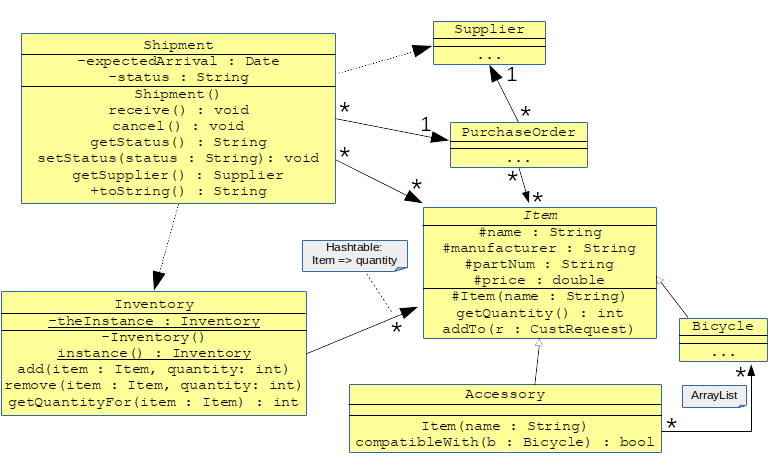
\includegraphics[width=.95\textwidth]{bikeClassDiag.png}
\caption{A first crack at converting CRC cards from Chapter~\ref{design1}'s
bicycle example into UML.}
\label{fig:bikeClassDiag}
\end{figure}

\index{purchase order@\texttt{Purchase Order}}
\index{supplier@\texttt{Supplier}}
We didn't actually write full CRC cards for all the classes in this design, but
that's okay: to complete \texttt{Shipment}, we can just sketch in temporary
placeholders for classes like \texttt{PurchaseOrder} and \texttt{Supplier}.

\index{accessory@\texttt{Accessory}}

The \texttt{Accessory} card from p.~\pageref{bikeCRC2} has a number of
``knows'' entries, though when we consider where to put them, we realize that
many of them will go in the abstract \texttt{Item} class. Only an
\texttt{ArrayList} of \texttt{Bicycle} objects seems appropriate as an inst var
for the \texttt{Accessory} subclass specifically, and that is what the diagram
shows. Since p.~\pageref{bikeCRC2} tells us that an \texttt{Accessory} ``knows
its compatible bicycle models,'' it seems appropriate for the class to support
a method like \texttt{.compatibleWith()} that returns a \texttt{boolean}
indicating whether the accessory in question is compatible with a particular
bike.

\index{Singleton pattern}
\index{design pattern!Singleton}
\index{inventory@\texttt{Inventory}}
Finally, our \texttt{Inventory} CRC card (also on p.~\pageref{bikeCRC2}) tells
us that in addition to the standard Singleton stuff, we need to be able to
\texttt{.add()} and \texttt{.remove()} quantities of items from the
\texttt{Inventory}, as well as get a current count of how many units of an
\texttt{Item} we have in stock. One way to implement this would be through a
\texttt{Hashtable} that maps each \texttt{Item} to an in-stock quantity, and
that is what Figure~\ref{fig:bikeClassDiag} shows.

I think you'll agree this is a pretty straightforward, though not completely
mechanical, process. CRC cards have already identified the lion's share of the
program's important static structure, and go a long way towards giving us a UML
class diagram from which we can write code.

\subsection{The Uno!\textsuperscript{\textregistered} game example, continued}
\index{Uno"!\textsuperscript{\textregistered}}

\index{card@\texttt{Card}}
\index{tree}
Now let's work on the Uno!\textsuperscript{\textregistered} example from the
CRC cards on pp.~\pageref{unoCRC1}--\pageref{unoCRC2}. We'll break this up into
two UML diagrams, one for the principal classes
(Figure~\ref{fig:unoClassDiag}), and the other for the \texttt{Card}
inheritance hierarchy (Figure~\ref{fig:unoCardHier}).

\index{simulation@\texttt{Simulation}}
\index{game@\texttt{Game}}
\index{play@\texttt{.play()}}
The CRC cards didn't explicitly say that \texttt{Simulation} would be our
\texttt{main()} class, but it's as good a choice as any, so that's what's
reflected in the diagram (bottom-left). All the ``knows'' have been given inst
vars. The \texttt{Simulation} will instantiate lots of \texttt{Game} objects:
one for each of the 50,000 games in the match, to be precise. Each
\texttt{Game}'s \texttt{.play()} method will simulate a single game to
completion, and return an array of the scores to add to each player's
cumulative total (held in the \texttt{Simulation} class). Btw,
we could have made \texttt{Simulation} a Singleton, and given it non-static
inst vars. Your call.

\subsubsection{The ``double dispatch'' technique}
\index{double dispatch}
\index{advanceToNextPlayer@\texttt{\texttt{.advanceToNextPlayer()}}}
\index{performCardEffect@\texttt{.performCardEffect()}}

The \texttt{Game} CRC card (middle of p.\pageref{unoCRC2}) tells us that it
must maintain the current player and the direction of play at all times. These
two bits of information are represented as inst vars in the second compartment
of the class. \texttt{Game} also has methods on it to
\texttt{.advanceToNextPlayer()} and to \texttt{.reverseDirection()}. These can
be called by any other part of the program in order to modify the game's state.
Our plan is for different \texttt{Card} subclasses to invoke these methods to
carry out their special effects: see the \texttt{.performCardEffect()} method
on the abstract \texttt{Card} class in the upper-left corner.

This technique is referred to as \textbf{double dispatch}, and it can be
disorienting at first. In double dispatch, you call a method on object A,
passing it another object B as an argument. Object A's method then, in addition
to whatever else it might need to do, will call method(s) on B.

\begin{figure}[ht]
\centering
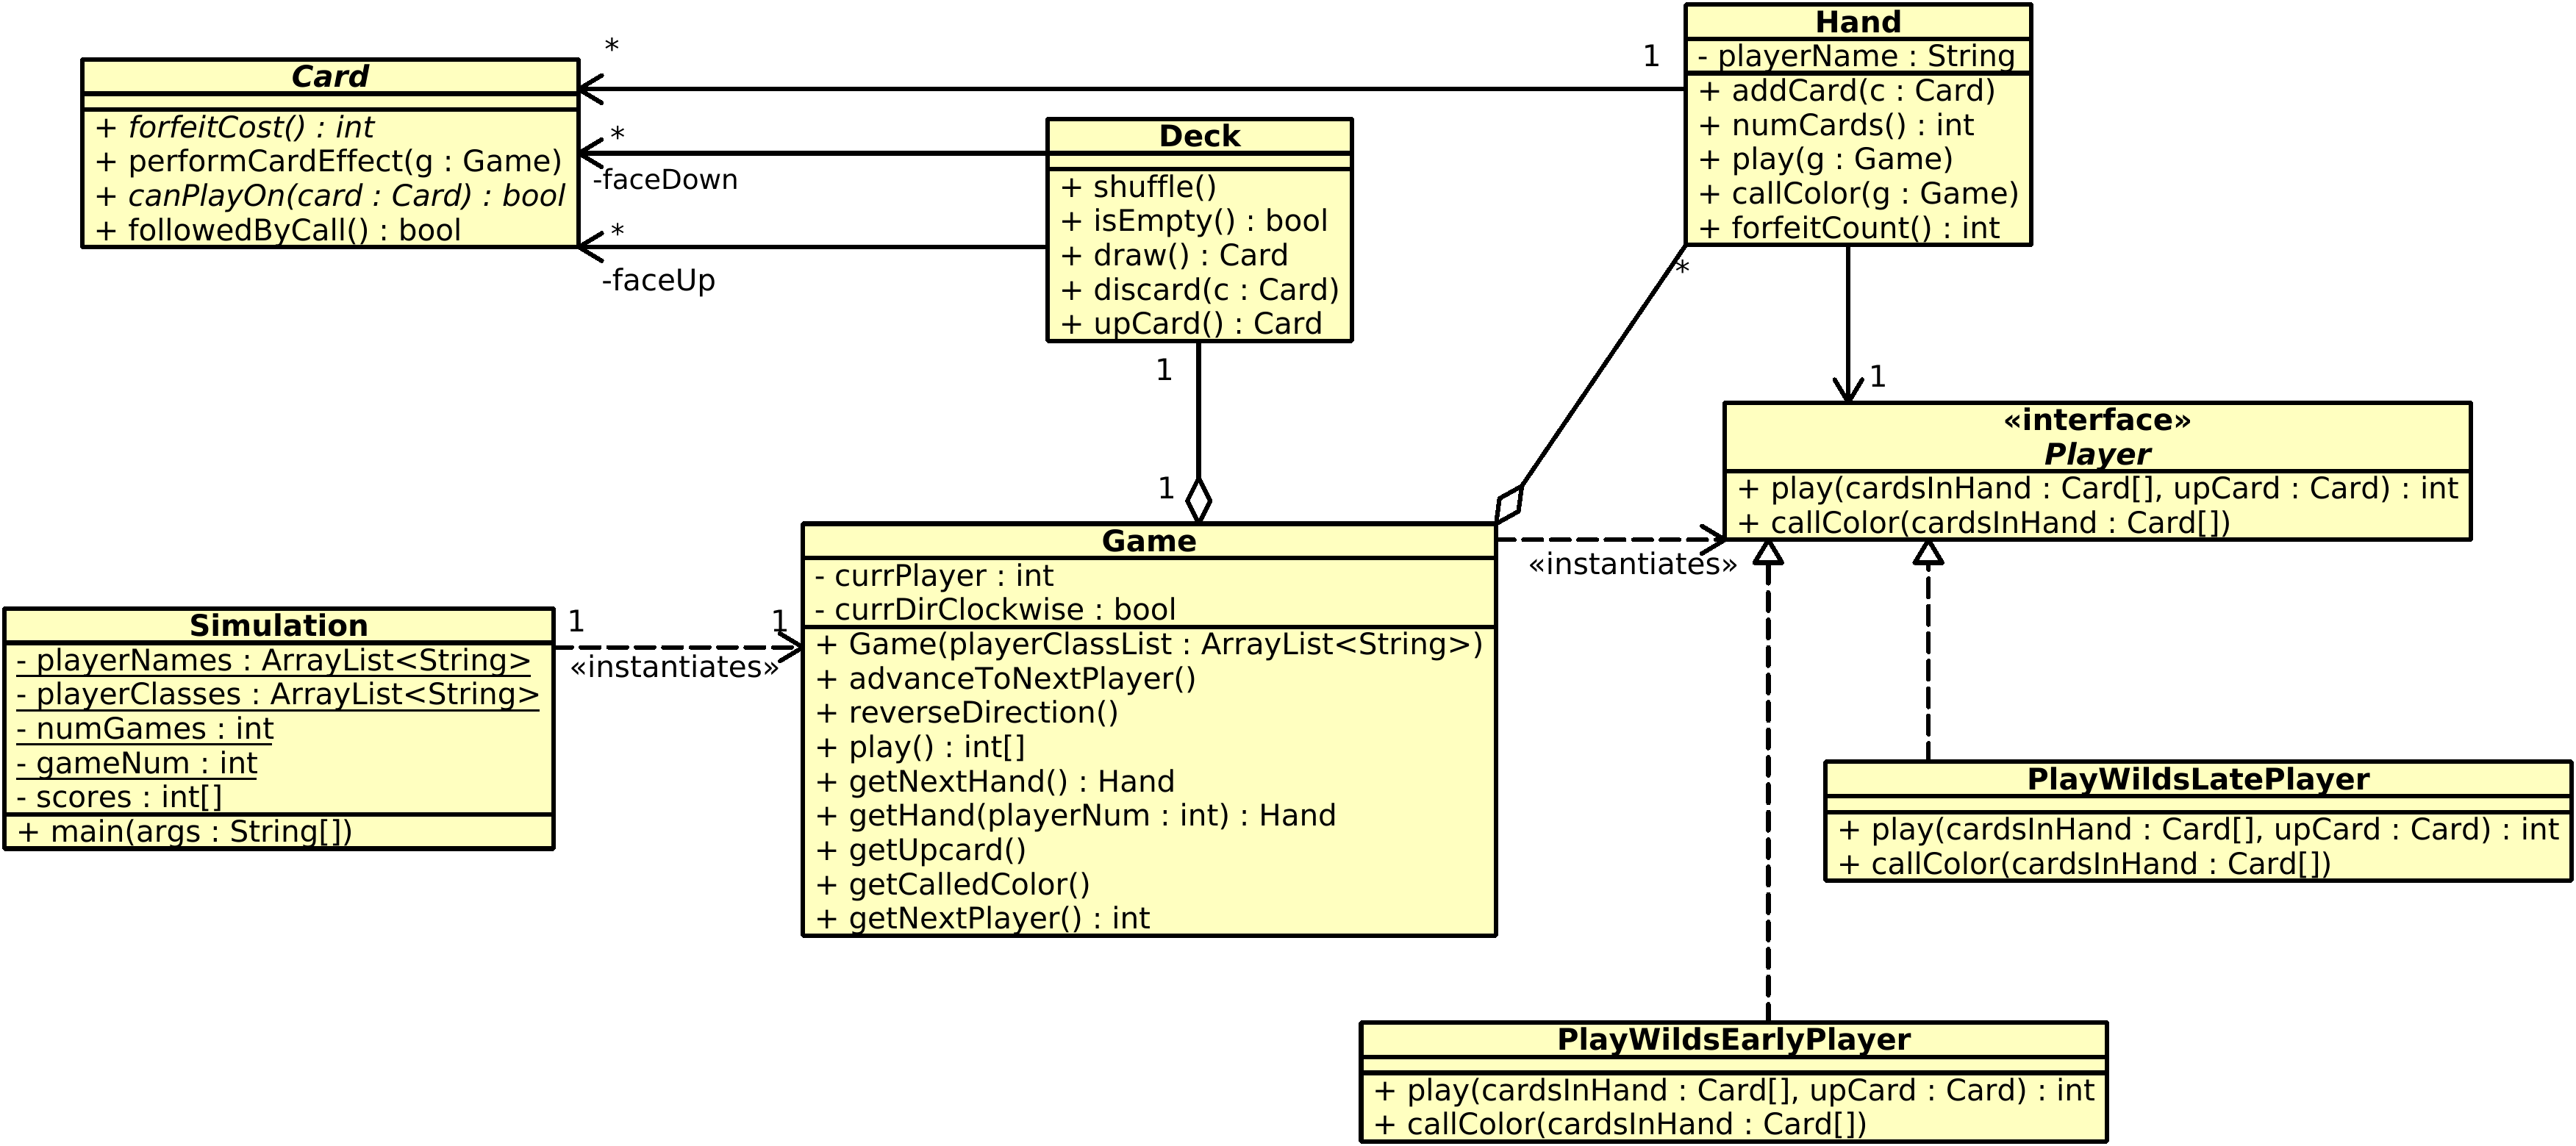
\includegraphics[width=1\textwidth]{UnoClassDiagram.png}
\medskip
\caption{A first cut at converting CRC cards from Chapter~\ref{design1}'s
Uno example into UML.}
\label{fig:unoClassDiag}
\end{figure}

\index{player@\texttt{Player} (Uno"! example)}
\index{hand@\texttt{Hand}}
\index{reverseCard@\texttt{ReverseCard}}
\index{play@\texttt{.play()}}
\index{getUpCard@\texttt{.getUpCard()}}
\index{performCardEffect@\texttt{.performCardEffect()}}
\index{sequence diagram}
Figure~\ref{fig:doubleDispatchUno} shows this in action for the Uno game. In
this scenario, the \texttt{Game} object determines that the next player is \#3,
and therefore instructs the third \texttt{Hand} to \texttt{.play()} a card.
\textbf{Note that \texttt{g} passes \texttt{h3} the argument ``\texttt{this}''
in the call to \texttt{.play()}.} That's how double dispatch works:
\texttt{h3}'s \texttt{.play()} method now has possession of the \texttt{Game}
object \texttt{g}, which it can call methods on and/or pass around further. In
this case it does both: first, \texttt{h3} turns around and calls
\texttt{.getUpCard()} on \texttt{g}, to find out what the up card is. Then,
when it passes that \texttt{up} card along to \texttt{p3}'s \texttt{.play()}
method, and learns that the \texttt{Player} algorithm chooses to play card \#7
from her hand (a blue reverse), it calls \texttt{.performCardEffect()} on that
\texttt{ReverseCard}. The \texttt{Card} object \texttt{c} now also has
possession of the \texttt{Game} object, and can tell it to do the two things
required: reverse the direction of play, and then advance to the next player's
turn. Other types of cards would do different things instead, as described
in the next section.

\index{double dispatch}
\begin{figure}[hb]
\centering
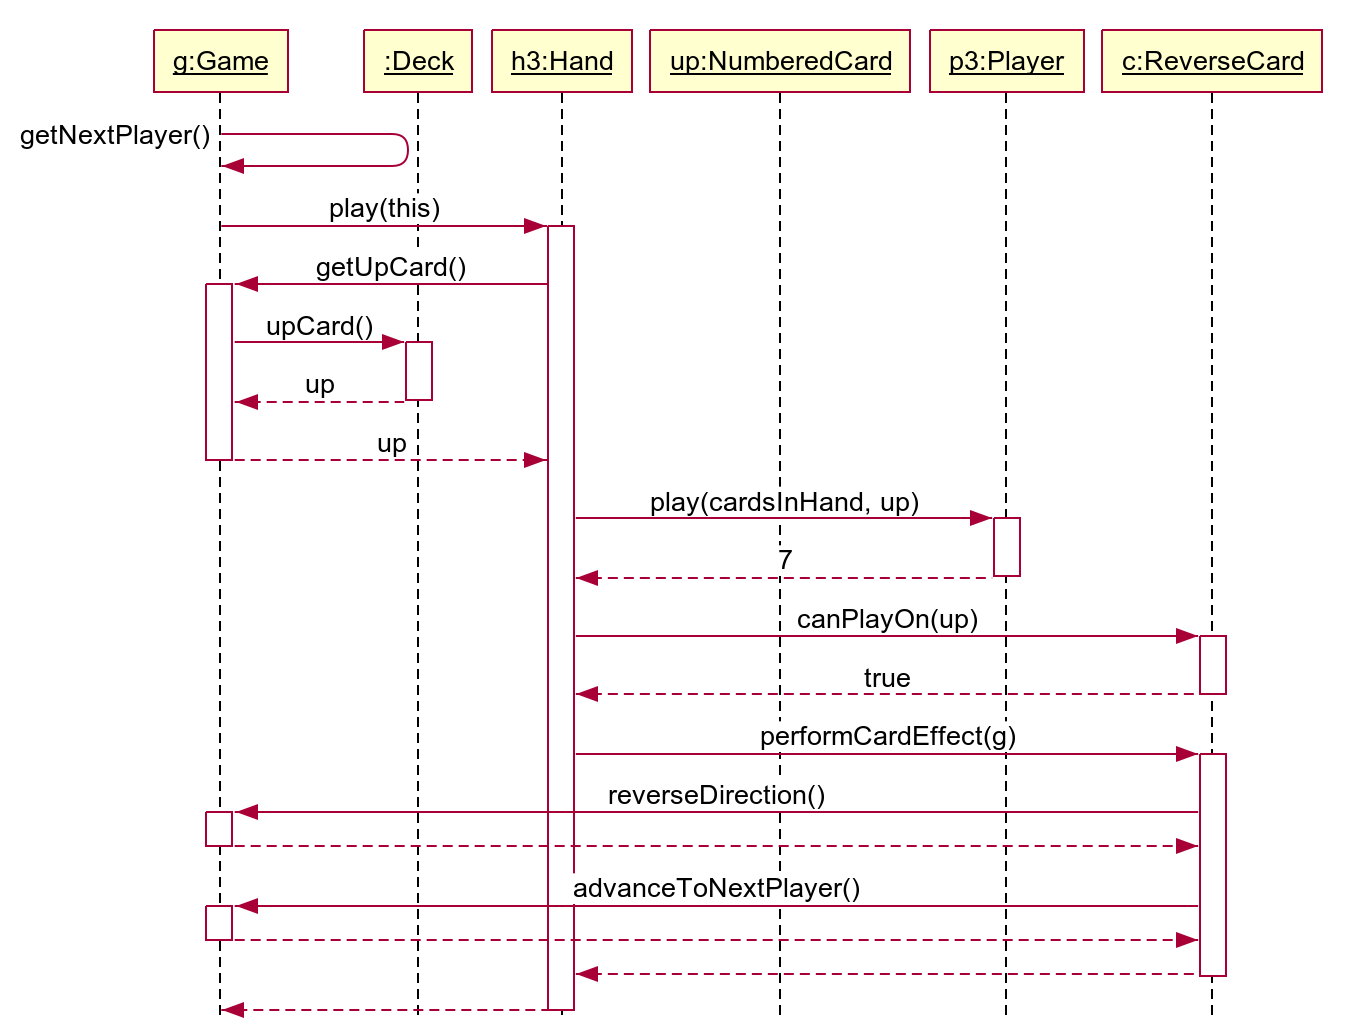
\includegraphics[width=1\textwidth]{doubleDispatchUno.png}
\medskip
\caption{An illustration of the double dispatch technique.}
\label{fig:doubleDispatchUno}
\end{figure}

\index{deck@\texttt{Deck}}
Back to Figure~\ref{fig:unoClassDiag}. We see that the \texttt{Deck} class --
whose CRC card was given on p.~\pageref{unoCRC2} -- contains \texttt{two}
collections of \texttt{Card} objects, one to hold a sequence of face-down cards
and one for the face-up cards. The rest of this class is self-explanatory.

\index{hand@\texttt{Hand}}
\texttt{Hand} objects each hold on to a list of \texttt{Card}s, of course, as
well as the corresponding player's name for good measure (which wasn't on the
CRC card). It also maintains an inst var to a ``\texttt{Player}'': this is the
creation by each of Stephen's students that implements the \texttt{Player}
interface and thus provides an algorithm for choosing cards and colors. Two
example players have been shown: one that plays wild cards as soon as it can,
and another that holds them until forced to. (Surprisingly, to me anyway, the
former outperformed the latter in most simulated games.)

\subsubsection{The \texttt{Card} class hierarchy}
\index{inheritance hierarchy}
\index{tree}
\index{card@\texttt{Card}}

Finally, let's figure out the \texttt{Card} class and its subclasses. It's a
bit tricky. One might think that a \texttt{Card} having a ``\texttt{number}''
is a no-brainer...except that not all cards \textit{have} numbers (like Skips
or Draw 2's.) Very well, then, at least all \texttt{Card}s have a
\textit{color}, you say...except that wild cards don't have that either.

\begin{figure}[ht]
\centering
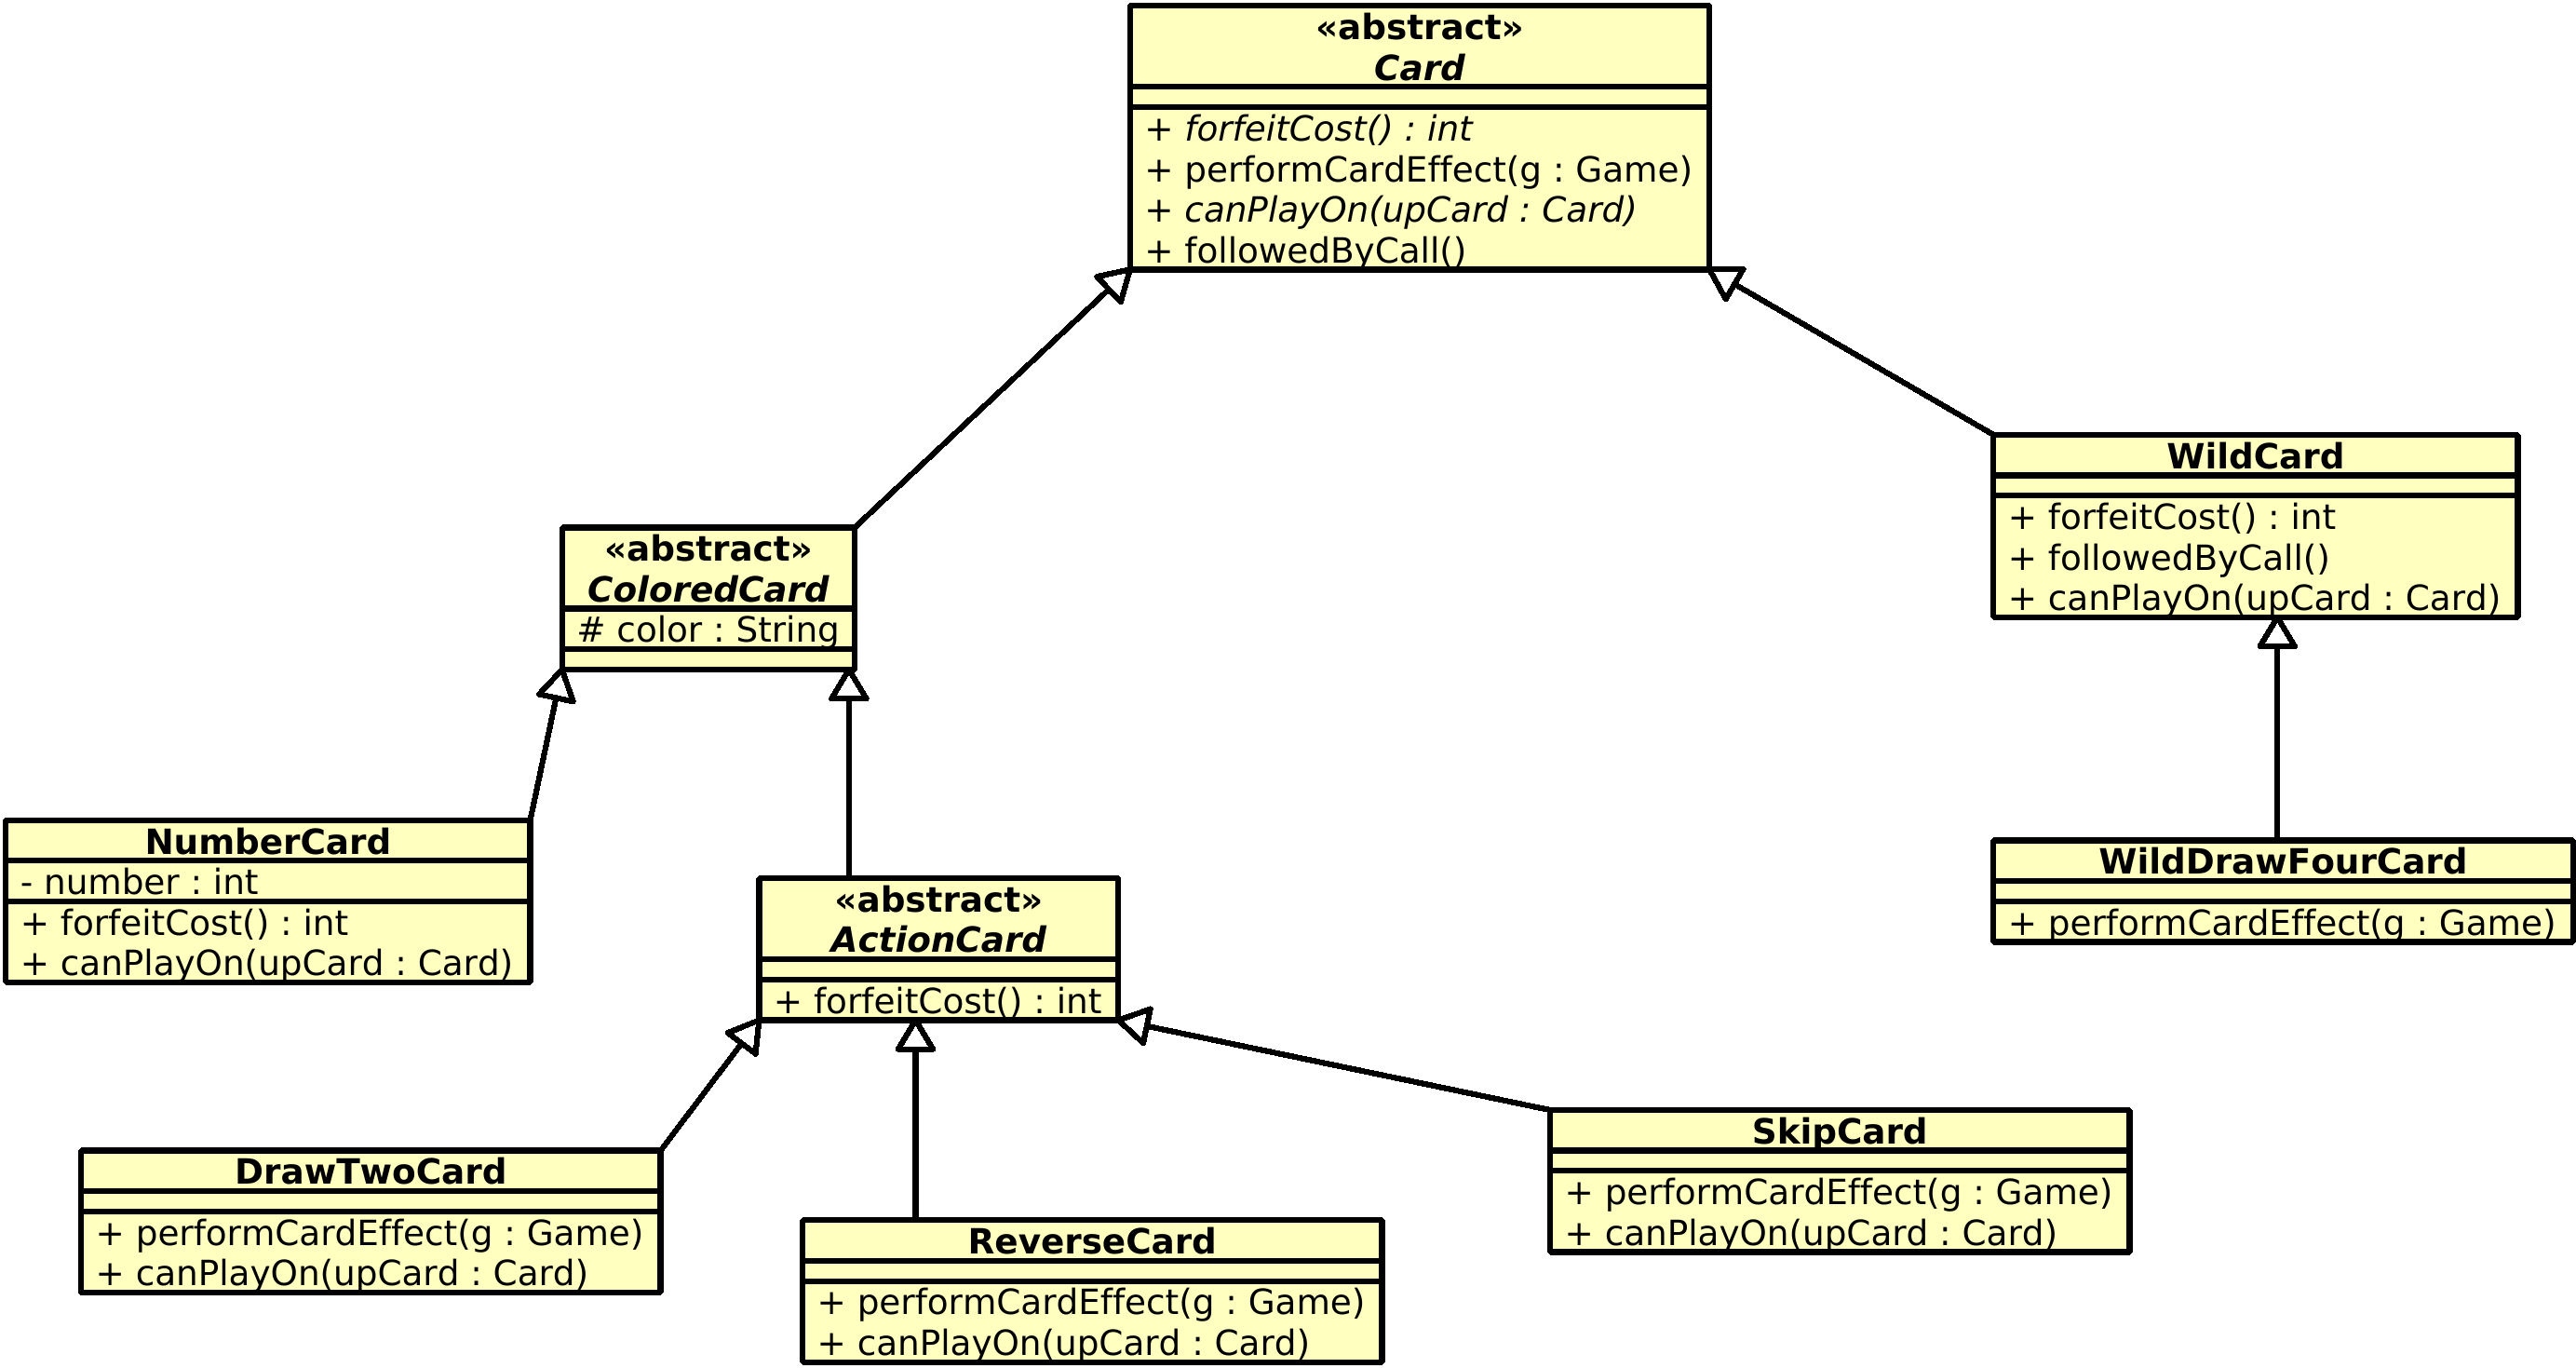
\includegraphics[width=1\textwidth]{UnoClassHierarchy.png}
\medskip
\caption{The \texttt{Card} class hierarchy from Chapter~\ref{design1}'s
Uno game example.}
\label{fig:unoCardHier}
\end{figure}

\index{abstract class}
\index{card@\texttt{Card}}
\index{reverseCard@\texttt{ReverseCard}}
\index{drawTwoCard@\texttt{DrawTwoCard}}
\index{skipCard@\texttt{SkipCard}}
\index{wildCard@\texttt{WildCard}}
\index{wildDrawFourCard@\texttt{WildDrawFourCard}}
\index{actionCard@\texttt{ActionCard}}
\index{coloredCard@\texttt{ColoredCard}}

\index{isa association@``is-a'' association}
\index{association!is-a@``is-a''}
\index{inheritance!top-down (interface)}
The trick is to recognize when there are commonalities between card types, and
to infer the presence of appropriate \textit{abstract} classes.
Figure~\ref{fig:unoCardHier} gives the idea. All of the associations here are
top-down inheritance (``is-a''). In addition to all the concrete \texttt{Card}
types you'd expect -- \texttt{DrawTwoCard}, \texttt{ReverseCard},
\texttt{WildCard}, \textit{etc.} -- we have created abstract
\texttt{ColoredCard} and \texttt{ActionCard} classes.

But isn't this overkill, you might ask? It is not, for the following reason:
each piece of information is now in only one place. For example, all numbered
cards \textit{and} ``action cards'' have a color, but wilds (of either variety)
do not. Therefore, it makes sense to define the \texttt{color} inst var in the
superclass of all the \texttt{Card} types that have colors. It shouldn't be in
the \texttt{Card} class itself -- that's too general, since not all
\texttt{Cards} have colors. And it shouldn't be in the \texttt{NumberedCard}
class -- that's too specific, since more than just numbered cards have colors.
By similar logic, only the \texttt{NumberedCard} class should have an
\texttt{int} inst var.

\index{actionCard@\texttt{ActionCard}}
\index{forfeitCost@\texttt{.forfeitCost()}}

Furthermore, since all ``action cards'' have the same forfeit cost (20~points)
it is appropriate to define a (non-abstract) \texttt{.forfeitCost()} method in
the (abstract) \texttt{ActionCard} class. That way, \texttt{SkipCard},
\texttt{ReverseCard}, and \texttt{DrawTwoCard} don't need to override it.

\index{wildCard@\texttt{WildCard}}
\index{wildDrawFourCard@\texttt{WildDrawFourCard}}
\index{performCardEffect@\texttt{.performCardEffect()}}

Note that \texttt{WildCard} is a concrete class, even though it has a subclass.
This is perfectly okay (in Java), and necessary since there are indeed ordinary
wild cards in the deck. Both types of wilds have the same forfeit cost
(50~points) and both require the player to call a color, but the Draw 4 variety
obviously has a different effect on the game, and therefore provides its own
\texttt{.performCardEffect()} method that overrides that of the
\texttt{WildCard} superclass (and the \texttt{Card} superclass).


\section{Evaluating a design}

I end this chapter by giving a few simple guidelines for sanity-checking your
design once you've gotten this far. Again, there is no one ``right way'' to
design a program, but there are plenty of wrong ways, and some of them are easy
to spot.

Here's my super short ``must-do'' checklist:

\index{encapsulation}
\index{responsibilities}
\index{cohesive (highly)}
\begin{compactenum}
\itemsep.1em
\item Each class represents a \textbf{crisp} and \textbf{coherent} entity.
\item Each class does \textbf{one thing} well.
\item Responsibilities are \textbf{distributed} over the entire design.
\item There is evidence of \textbf{encapsulation}.
\end{compactenum}

The first item on the list is somewhat intangible, but oh-so-important. It
basically means that the meaning and purpose of each class should be natural
and easy to describe. If you find yourself struggling to articulate what
specific type of entity one of your classes actually represents, rethink it.

\index{god class@``god class''}
The second item involves a very common pitfall for beginning designers: having
\textit{too few classes, each of which does too much.}\footnote{I have a theory
that this is normally due to simple laziness in creating new files, but I've
never seen that proven.} There's a funny name for a class that does too much:
it's called a ``\textbf{god class}'' (no joke.) Very often, I see students
creating designs that on the surface seem to have several collaborating
classes, but which in actuality have all the real functionality in one god
class while the others serve merely as data containers.

Strive instead to have each class do only one self-contained job, and to do it
well. Remember: the larger your classes are, and the more tasks each one
encompasses, the less encapsulated your program is bound to be.

\index{sequence diagram}
Related to this is the third item, which is that when your program is in
operation, most of its important responsibilities should be \textit{shared}
between the different classes. This is exposed clearly on sequence diagrams:
if you find that most of your arrows are emanating from a single vertical line,
that's a bad sign. If you look at the Uno design, you'll see that any
significant operation -- like a player actually taking her turn -- involves
many classes operating in tandem: \texttt{Game}, \texttt{Deck}, \texttt{Hand},
a \texttt{Player} implementation, and some subclass of \texttt{Card}. This is A
Good Thing.\texttrademark

\index{association}
Finally, for each class, you want to scrutinize its list of inst vars (both
those in the second compartment and those implied by associations) and its
methods and make sure they all ``fit together'' well. They should all make
sense for that type, and the data and behavior should go hand in hand. Each
class's design decisions should be cleanly insulated from others. Ideally, when
you look at your design, you should see a picture like the right-hand side of
Figure~\ref{fig:dependencies} (p.~\pageref{fig:dependencies}), not the left.
